\documentclass{standalone}
\usepackage{tikz}
\usetikzlibrary{patterns, positioning}
\usepackage[sfdefault]{ClearSans} %% option 'sfdefault' activates Clear Sans as the default text font
\usepackage[T1]{fontenc}

\begin{document}
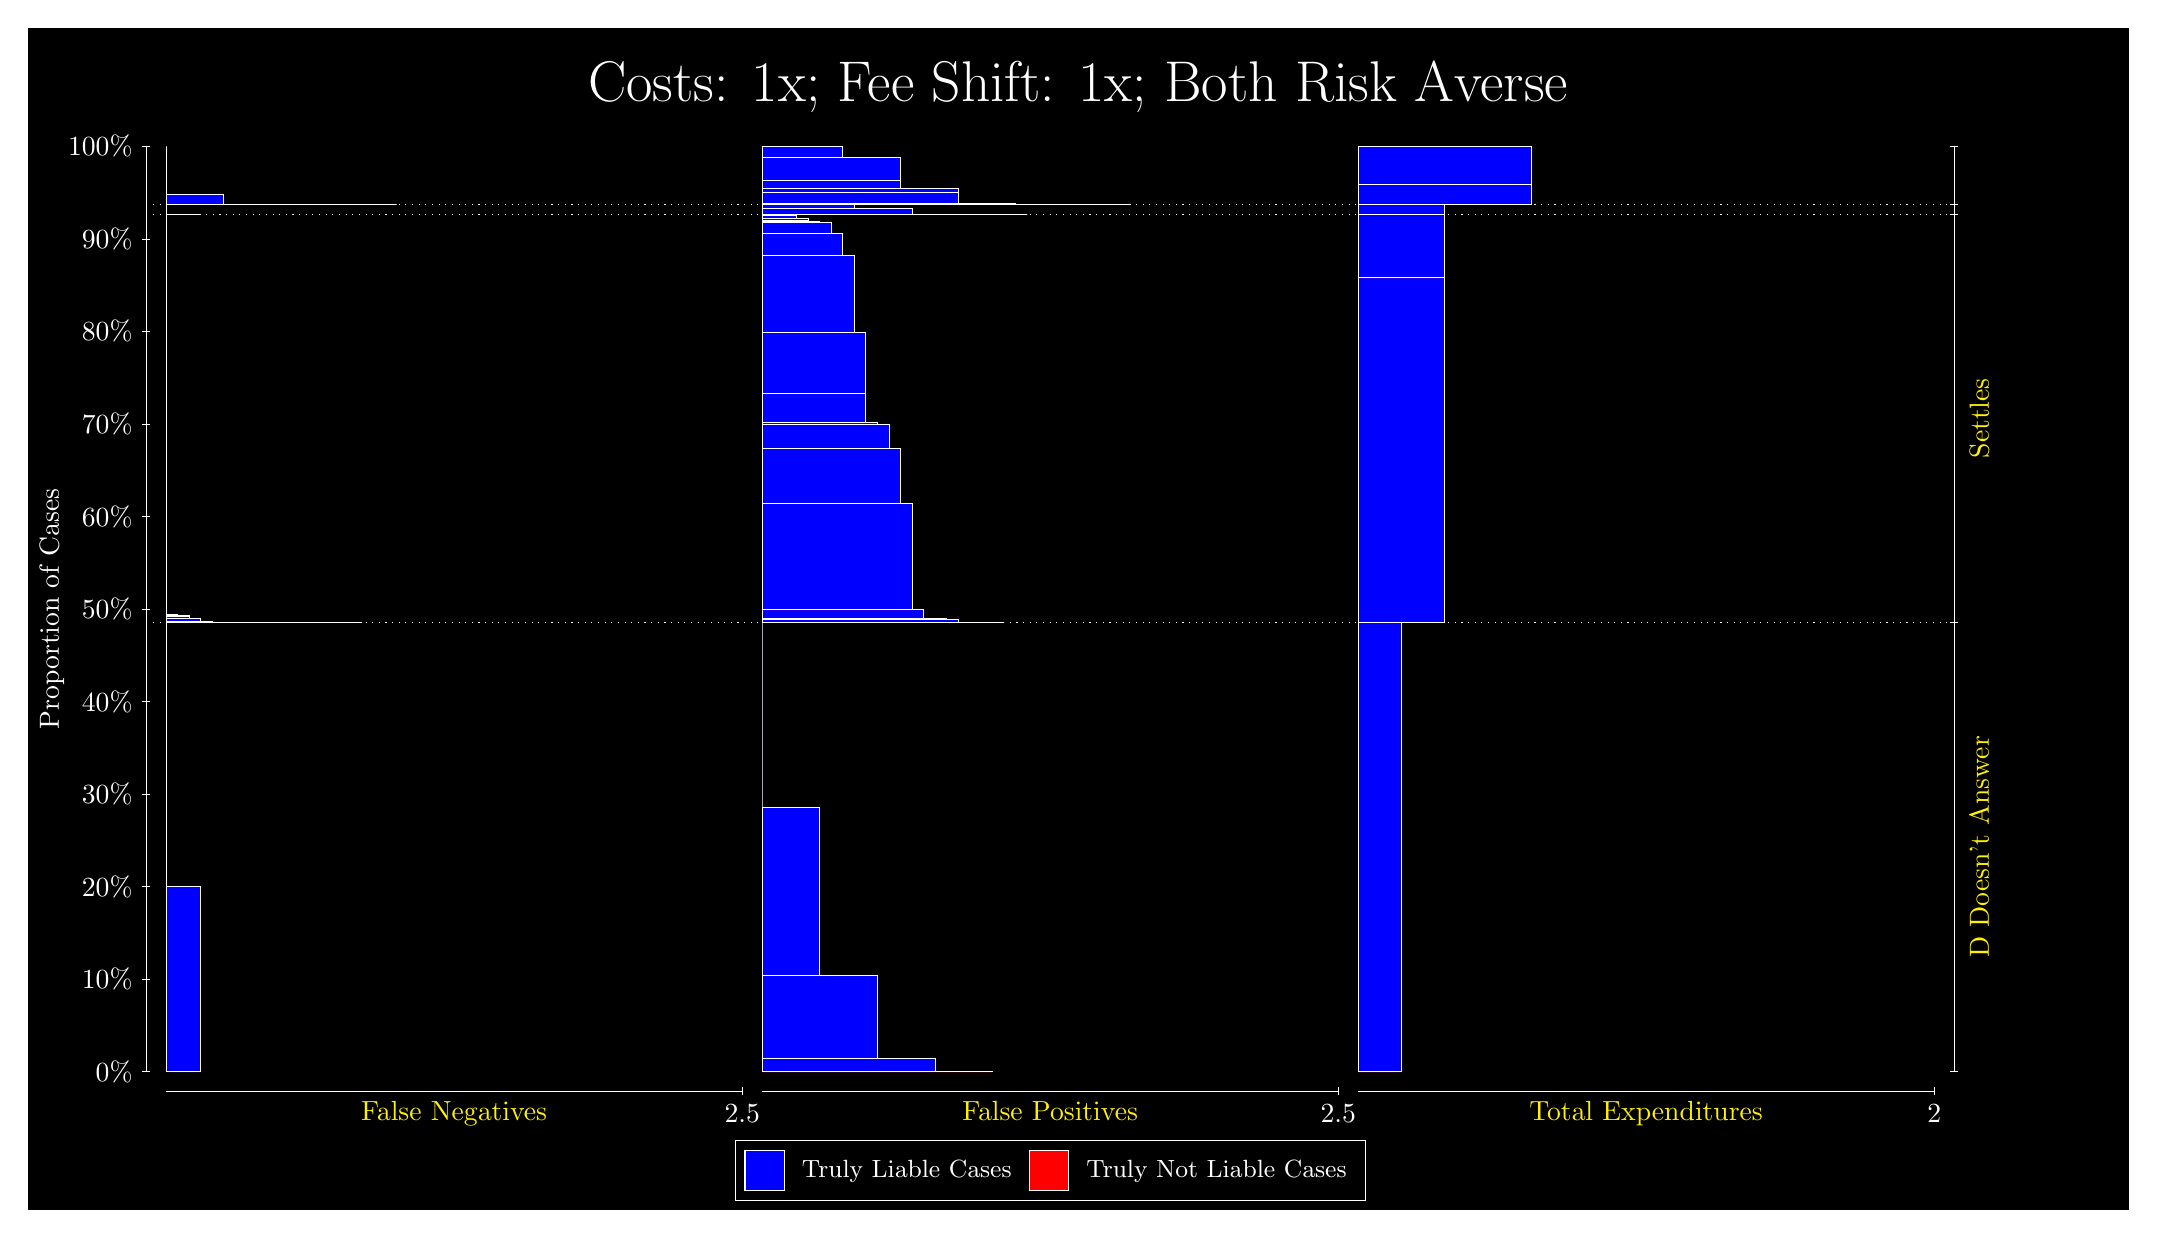
\begin{tikzpicture}
\draw[fill=black] (0,0) rectangle (26.667,15);
\draw[text=white] (0,13.5) rectangle (26.667,15) node[midway] {\huge Costs: 1x; Fee Shift: 1x; Both Risk Averse};
\draw[white, very thin] (1.5,1.75) -- (1.5,13.5);
\node[rotate=90, text=white, anchor=center] at (0.3, 7.625) {Proportion of Cases};
\draw[white, very thin] (1.45,1.75) -- (1.55,1.75);
\node[text=white, anchor=east] at (1.45, 1.75) {0\%};
\draw[white, very thin] (1.45,2.925) -- (1.55,2.925);
\node[text=white, anchor=east] at (1.45, 2.925) {10\%};
\draw[white, very thin] (1.45,4.1) -- (1.55,4.1);
\node[text=white, anchor=east] at (1.45, 4.1) {20\%};
\draw[white, very thin] (1.45,5.275) -- (1.55,5.275);
\node[text=white, anchor=east] at (1.45, 5.275) {30\%};
\draw[white, very thin] (1.45,6.45) -- (1.55,6.45);
\node[text=white, anchor=east] at (1.45, 6.45) {40\%};
\draw[white, very thin] (1.45,7.625) -- (1.55,7.625);
\node[text=white, anchor=east] at (1.45, 7.625) {50\%};
\draw[white, very thin] (1.45,8.8) -- (1.55,8.8);
\node[text=white, anchor=east] at (1.45, 8.8) {60\%};
\draw[white, very thin] (1.45,9.975) -- (1.55,9.975);
\node[text=white, anchor=east] at (1.45, 9.975) {70\%};
\draw[white, very thin] (1.45,11.15) -- (1.55,11.15);
\node[text=white, anchor=east] at (1.45, 11.15) {80\%};
\draw[white, very thin] (1.45,12.325) -- (1.55,12.325);
\node[text=white, anchor=east] at (1.45, 12.325) {90\%};
\draw[white, very thin] (1.45,13.5) -- (1.55,13.5);
\node[text=white, anchor=east] at (1.45, 13.5) {100\%};

\draw[white, very thin] (24.457,1.75) -- (24.457,13.5);
\draw[white, very thin] (24.407,1.75) -- (24.507,1.75);
\node[anchor=west] at (24.407, 1.75) {};
\draw[white, very thin] (24.407,7.4568) -- (24.507,7.4568);
\node[anchor=west] at (24.407, 7.4568) {};
\draw[white, very thin] (24.407,12.636) -- (24.507,12.636);
\node[anchor=west] at (24.407, 12.636) {};
\draw[white, very thin] (24.407,12.763) -- (24.507,12.763);
\node[anchor=west] at (24.407, 12.763) {};
\draw[white, very thin] (24.407,13.5) -- (24.507,13.5);
\node[anchor=west] at (24.407, 13.5) {};

\draw[white, very thin, fill=blue] (1.75,1.75) rectangle (2.1891,4.0978);
\draw[white, very thin, fill=red] (1.75,4.0978) rectangle (1.75,4.0978);
\draw[white, very thin, fill=blue] (1.75,4.0978) rectangle (1.75,7.4568);
\draw[white, very thin, fill=blue] (1.75,7.4568) rectangle (4.2384,7.4568);
\draw[white, very thin, fill=blue] (1.75,7.4568) rectangle (3.6529,7.4568);
\draw[white, very thin, fill=blue] (1.75,7.4568) rectangle (3.5065,7.4568);
\draw[white, very thin, fill=blue] (1.75,7.4568) rectangle (3.3602,7.4568);
\draw[white, very thin, fill=blue] (1.75,7.4568) rectangle (3.0674,7.4568);
\draw[white, very thin, fill=blue] (1.75,7.4568) rectangle (2.921,7.4568);
\draw[white, very thin, fill=blue] (1.75,7.4568) rectangle (2.7746,7.4568);
\draw[white, very thin, fill=blue] (1.75,7.4568) rectangle (2.6283,7.4568);
\draw[white, very thin, fill=blue] (1.75,7.4568) rectangle (2.4819,7.4584);
\draw[white, very thin, fill=blue] (1.75,7.4584) rectangle (2.3355,7.4646);
\draw[white, very thin, fill=blue] (1.75,7.4646) rectangle (2.1891,7.5062);
\draw[white, very thin, fill=blue] (1.75,7.5062) rectangle (2.0428,7.5353);
\draw[white, very thin, fill=blue] (1.75,7.5353) rectangle (2.0428,7.5503);
\draw[white, very thin, fill=blue] (1.75,7.5503) rectangle (1.8964,7.5511);
\draw[white, very thin, fill=red] (1.75,7.5511) rectangle (1.75,7.5511);
\draw[white, very thin, fill=blue] (1.75,7.5511) rectangle (1.75,12.636);
\draw[white, very thin, fill=blue] (1.75,12.636) rectangle (2.1891,12.636);
\draw[white, very thin, fill=red] (1.75,12.636) rectangle (1.75,12.636);
\draw[white, very thin, fill=blue] (1.75,12.636) rectangle (1.75,12.763);
\draw[white, very thin, fill=blue] (1.75,12.763) rectangle (4.6775,12.763);
\draw[white, very thin, fill=blue] (1.75,12.763) rectangle (3.9457,12.763);
\draw[white, very thin, fill=blue] (1.75,12.763) rectangle (3.2138,12.768);
\draw[white, very thin, fill=blue] (1.75,12.768) rectangle (2.4819,12.897);
\draw[white, very thin, fill=red] (1.75,12.897) rectangle (1.75,12.897);
\draw[white, very thin, fill=blue] (1.75,12.897) rectangle (1.75,13.5);
\draw[white, very thin, fill=red] (9.3189,1.75) rectangle (12.246,1.75);
\draw[white, very thin, fill=blue] (9.3189,1.75) rectangle (12.246,1.7516);
\draw[white, very thin, fill=blue] (9.3189,1.7516) rectangle (11.515,1.9134);
\draw[white, very thin, fill=blue] (9.3189,1.9134) rectangle (10.783,2.9737);
\draw[white, very thin, fill=blue] (9.3189,2.9737) rectangle (10.051,5.109);
\draw[white, very thin, fill=blue] (9.3189,5.109) rectangle (9.3189,7.4568);
\draw[white, very thin, fill=red] (9.3189,7.4568) rectangle (12.393,7.4568);
\draw[white, very thin, fill=blue] (9.3189,7.4568) rectangle (12.393,7.4568);
\draw[white, very thin, fill=red] (9.3189,7.4568) rectangle (12.1,7.4568);
\draw[white, very thin, fill=blue] (9.3189,7.4568) rectangle (12.1,7.457);
\draw[white, very thin, fill=red] (9.3189,7.457) rectangle (11.807,7.457);
\draw[white, very thin, fill=blue] (9.3189,7.457) rectangle (11.807,7.4987);
\draw[white, very thin, fill=blue] (9.3189,7.4987) rectangle (11.661,7.5091);
\draw[white, very thin, fill=red] (9.3189,7.5091) rectangle (11.515,7.5091);
\draw[white, very thin, fill=blue] (9.3189,7.5091) rectangle (11.515,7.5102);
\draw[white, very thin, fill=blue] (9.3189,7.5102) rectangle (11.368,7.6172);
\draw[white, very thin, fill=red] (9.3189,7.6172) rectangle (11.222,7.6172);
\draw[white, very thin, fill=blue] (9.3189,7.6172) rectangle (11.222,8.9673);
\draw[white, very thin, fill=blue] (9.3189,8.9673) rectangle (11.075,9.6673);
\draw[white, very thin, fill=blue] (9.3189,9.6673) rectangle (10.929,9.9698);
\draw[white, very thin, fill=blue] (9.3189,9.9698) rectangle (10.783,9.991);
\draw[white, very thin, fill=blue] (9.3189,9.991) rectangle (10.636,10.361);
\draw[white, very thin, fill=red] (9.3189,10.361) rectangle (10.636,10.361);
\draw[white, very thin, fill=blue] (9.3189,10.361) rectangle (10.636,11.135);
\draw[white, very thin, fill=blue] (9.3189,11.135) rectangle (10.49,12.115);
\draw[white, very thin, fill=blue] (9.3189,12.115) rectangle (10.344,12.396);
\draw[white, very thin, fill=blue] (9.3189,12.396) rectangle (10.197,12.541);
\draw[white, very thin, fill=blue] (9.3189,12.541) rectangle (10.051,12.542);
\draw[white, very thin, fill=blue] (9.3189,12.542) rectangle (9.9044,12.557);
\draw[white, very thin, fill=blue] (9.3189,12.557) rectangle (9.9044,12.586);
\draw[white, very thin, fill=blue] (9.3189,12.586) rectangle (9.758,12.628);
\draw[white, very thin, fill=blue] (9.3189,12.628) rectangle (9.6116,12.634);
\draw[white, very thin, fill=blue] (9.3189,12.634) rectangle (9.4652,12.636);
\draw[white, very thin, fill=blue] (9.3189,12.636) rectangle (9.3189,12.636);
\draw[white, very thin, fill=red] (9.3189,12.636) rectangle (12.686,12.636);
\draw[white, very thin, fill=blue] (9.3189,12.636) rectangle (12.686,12.636);
\draw[white, very thin, fill=blue] (9.3189,12.636) rectangle (11.954,12.638);
\draw[white, very thin, fill=blue] (9.3189,12.638) rectangle (11.222,12.718);
\draw[white, very thin, fill=blue] (9.3189,12.718) rectangle (10.49,12.762);
\draw[white, very thin, fill=blue] (9.3189,12.762) rectangle (9.758,12.763);
\draw[white, very thin, fill=red] (9.3189,12.763) rectangle (14.003,12.763);
\draw[white, very thin, fill=blue] (9.3189,12.763) rectangle (14.003,12.763);
\draw[white, very thin, fill=red] (9.3189,12.763) rectangle (13.271,12.763);
\draw[white, very thin, fill=blue] (9.3189,12.763) rectangle (13.271,12.763);
\draw[white, very thin, fill=red] (9.3189,12.763) rectangle (12.539,12.763);
\draw[white, very thin, fill=blue] (9.3189,12.763) rectangle (12.539,12.781);
\draw[white, very thin, fill=blue] (9.3189,12.781) rectangle (11.807,12.911);
\draw[white, very thin, fill=red] (9.3189,12.911) rectangle (11.807,12.911);
\draw[white, very thin, fill=blue] (9.3189,12.911) rectangle (11.807,12.966);
\draw[white, very thin, fill=blue] (9.3189,12.966) rectangle (11.075,13.074);
\draw[white, very thin, fill=red] (9.3189,13.074) rectangle (11.075,13.074);
\draw[white, very thin, fill=blue] (9.3189,13.074) rectangle (11.075,13.366);
\draw[white, very thin, fill=blue] (9.3189,13.366) rectangle (10.344,13.366);
\draw[white, very thin, fill=blue] (9.3189,13.366) rectangle (10.344,13.495);
\draw[white, very thin, fill=blue] (9.3189,13.495) rectangle (9.6116,13.495);
\draw[white, very thin, fill=blue] (9.3189,13.495) rectangle (9.6116,13.5);
\draw[white, very thin, fill=blue] (9.3189,13.5) rectangle (9.3189,13.5);
\draw[white, very thin, fill=red] (16.888,1.75) rectangle (17.437,1.75);
\draw[white, very thin, fill=blue] (16.888,1.75) rectangle (17.437,7.4568);
\draw[white, very thin, fill=red] (16.888,7.4568) rectangle (17.986,7.4568);
\draw[white, very thin, fill=blue] (16.888,7.4568) rectangle (17.986,11.833);
\draw[white, very thin, fill=red] (16.888,11.833) rectangle (17.986,11.833);
\draw[white, very thin, fill=blue] (16.888,11.833) rectangle (17.986,12.636);
\draw[white, very thin, fill=red] (16.888,12.636) rectangle (17.986,12.636);
\draw[white, very thin, fill=blue] (16.888,12.636) rectangle (17.986,12.763);
\draw[white, very thin, fill=red] (16.888,12.763) rectangle (19.083,12.763);
\draw[white, very thin, fill=blue] (16.888,12.763) rectangle (19.083,13.019);
\draw[white, very thin, fill=red] (16.888,13.019) rectangle (19.083,13.019);
\draw[white, very thin, fill=blue] (16.888,13.019) rectangle (19.083,13.5);
\draw[white, dotted] (1.5,7.4568) -- (24.457,7.4568);
\draw[white, dotted] (1.5,12.636) -- (24.457,12.636);
\draw[white, dotted] (1.5,12.763) -- (24.457,12.763);
\draw[white, very thin] (1.75,1.5) -- (9.0689,1.5);
\node[text=yellow, anchor=north] at (5.4094, 1.5) {False Negatives};
\draw[white, very thin] (9.0689,1.45) -- (9.0689,1.55);
\node[text=white, anchor=north] at (9.0689, 1.45) {2.5};

\draw[white, very thin] (9.3189,1.5) -- (16.638,1.5);
\node[text=yellow, anchor=north] at (12.978, 1.5) {False Positives};
\draw[white, very thin] (16.638,1.45) -- (16.638,1.55);
\node[text=white, anchor=north] at (16.638, 1.45) {2.5};

\draw[white, very thin] (16.888,1.5) -- (24.207,1.5);
\node[text=yellow, anchor=north] at (20.547, 1.5) {Total Expenditures};
\draw[white, very thin] (24.207,1.45) -- (24.207,1.55);
\node[text=white, anchor=north] at (24.207, 1.45) {2};

\node[text=yellow, centered, rotate=90] at (24.777, 4.6034) {D Doesn't Answer};
\node[text=yellow, centered, rotate=90] at (24.777, 10.046) {Settles};



\draw (12.978300999999998,1.5) node[draw=none] (baseCoordinate) {};
\begin{scope}[align=center]
        \matrix[scale=0.5, draw=white, below=0.5cm of baseCoordinate, nodes={draw}, column sep=0.1cm]{
            \node[rectangle, draw, minimum width=0.5cm, minimum height=0.5cm, fill=blue] {}; &
            \node[draw=none, font=\small, text=white] (B) {Truly Liable Cases}; &
            \node[rectangle, draw, minimum width=0.5cm, minimum height=0.5cm, fill=red] {}; &
            \node[draw=none, font=\small, text=white] (B) {Truly Not Liable Cases}; \\
            };
\end{scope}

\end{tikzpicture}
\end{document}